\section{En trigonometría}

\label{1:sec:1}
En trigonometría el seno de un ángulo en un triángulo rectángulo se define como la razón entre
el cateto opuesto y la hipotenusa:\[f(x)=sin(x)\]
O también como la ordenada correspondiente a un punto que pertenece a una circunferencia unitaria
centrada en el origen (c=1):\[sin \alpha =a\]
En matemáticas el seno es la función continua y periódica obtenida al hacer variar la razón mencionada,
siendo una de las funciones trascendentes.
\begin{figure}[h]
\begin{center}
\includegraphics[scale=0.2]{images/seno.eps}
\end{center}
\caption{FuncionSeno}
\label{graph:3}
\end{figure}

\section{El seno en programación}
\label{1:sec:2}

  Normalmente todos los lenguajes de programación proveen una función
seno. También es normal en todos los lenguajes que el ángulo que recibe
la función deba pasarse en radianes.

  Esto es importante tenerlo en cuenta ya que si no podrían derivarse errores
por este concepto. Del mismo modo las calculadoras suelen aceptar el valor 
en grados o radianes, siendo necesario para ello (realizar dicho cálculo 
correctamente) activar un botón selector del tipo de grados (sexagesimales, 
centesimales o radianes) que se desea usar.

\begin{figure}[h]
\begin{center}
\includegraphics[scale=0.55]{images/ejemplo_seno.eps}
\end{center}
\caption{EjemploSeno}
\label{graph:4}
\end{figure}

Obsérvese como la escasa diferencia entre ambos valores resultantes podría pasar
desapercibida. Es necesario, por tanto, cuando sea conveniente pasar los grados 
a radianes o viceversa. Nótese que el símbolo $\pi$ es el número $\pi$

